$if(has-frontmatter)$
\frontmatter
$endif$
% ---------- Sampul ----------
\begin{titlepage}
\thispagestyle{empty}
\begin{tikzpicture}[remember picture, overlay]
  \node[anchor=south, inner sep=0pt, opacity=0.18] at (current page.south)
    {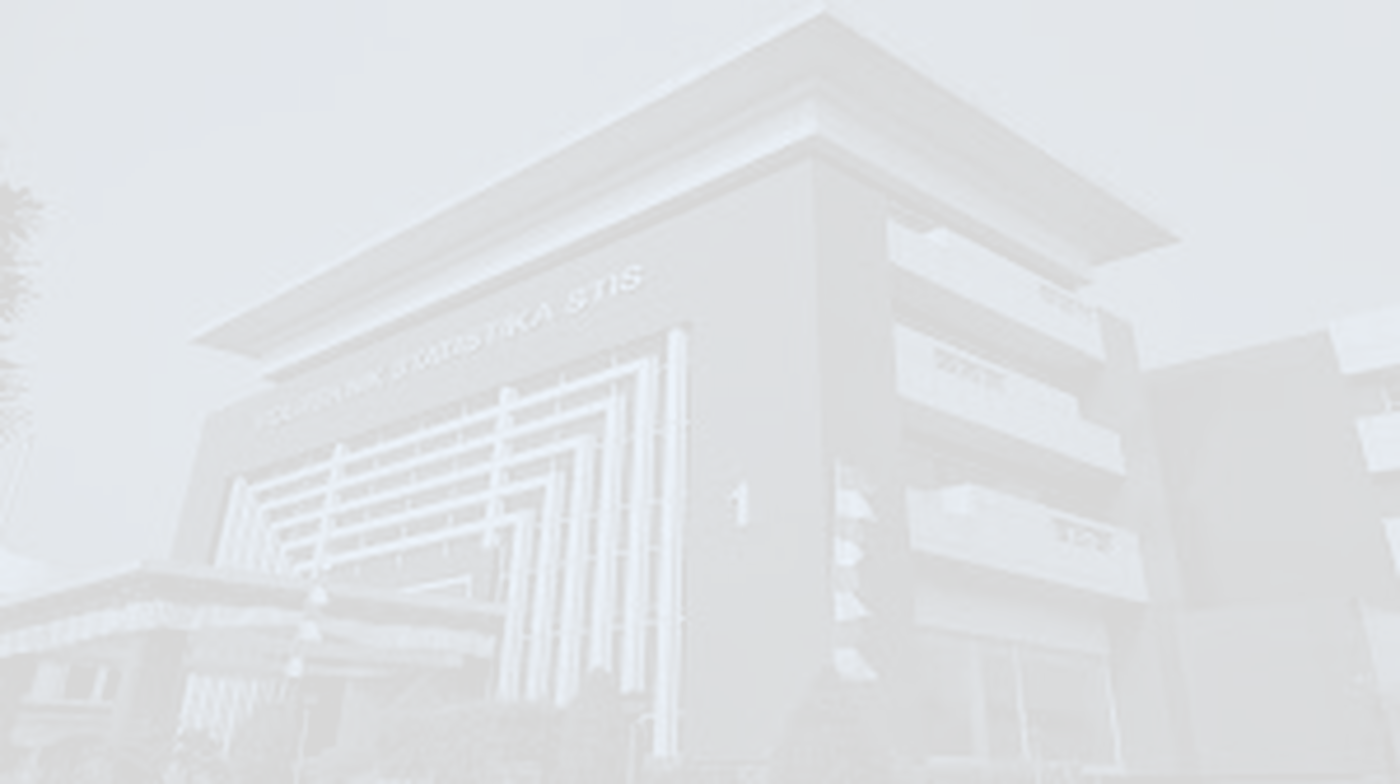
\includegraphics[width=\paperwidth]{gambar/gedung_bg.png}};
  \fill[bpsnavy] (current page.north west) -- ++(0,-9.2cm) --
        ($$(current page.north east)+(0,-6.4cm)$$) -- (current page.north east) -- cycle;
  \fill[bpsbiru] ($$(current page.north west)+(0,-9.2cm)$$) -- ++(0,-0.9cm) --
        ($$(current page.north east)+(0,-7.3cm)$$) -- ($$(current page.north east)+(0,-6.4cm)$$) -- cycle;
  \fill[bpsoranye] ($$(current page.north west)+(0,-10.1cm)$$) -- ++(0,-0.25cm) --
        ($$(current page.north east)+(0,-7.55cm)$$) -- ($$(current page.north east)+(0,-7.3cm)$$) -- cycle;
  \node[anchor=north west, inner sep=0pt] at ($$(current page.north west)+(2.2cm,-1.8cm)$$)
    {
\includegraphics[height=2.2cm]{gambar/logo_stis.png}};
  \node[anchor=north west, text=white, align=left, font=\sffamily] at
    ($$(current page.north west)+(5.2cm,-2.0cm)$$)
    {\Large\bfseries POLITEKNIK STATISTIKA STIS\\[4pt]\normalsize Buku Pedoman Paket R};
  \node[anchor=north west, text width=15cm, align=left, font=\sffamily] at
    ($$(current page.north west)+(2.2cm,-12.3cm)$$)
    {{\color{bpsoranye}\large\bfseries BUKU PEDOMAN}\\[10pt]
     {\color{bpsnavy}\fontsize{28}{34}\selectfont\bfseries\hyphenpenalty=10000\exhyphenpenalty=10000 $title$}\\[14pt]
     {\color{bpsbiru}\Large $subtitle$}};
  \fill[bpsnavy] ($$(current page.south west)+(0,3.4cm)$$) rectangle (current page.south east);
  \fill[bpsoranye] ($$(current page.south west)+(0,3.4cm)$$) rectangle
        ($$(current page.south east)+(0,3.55cm)$$);
  \node[anchor=west, text=white, align=left, font=\sffamily] at
    ($$(current page.south west)+(2.2cm,1.75cm)$$)
    {\large\bfseries $for(author)$$author$$sep$, $endfor$\\[3pt]
     \normalsize Untuk paket \texttt{modulstis} versi \versimodulstis{} \quad$$\cdot$$\quad $date$};
\end{tikzpicture}
\end{titlepage}

% ---------- Halaman hak cipta ----------
\thispagestyle{empty}
\vspace*{\fill}
{\small\color{abuteks}
\textbf{\color{bpsnavy}$title$}\\
$subtitle$\\[8pt]
Penyusun: $for(author)$$author$$sep$, $endfor$\\
Politeknik Statistika STIS, Jakarta\\[8pt]
Untuk paket \texttt{modulstis} versi \versimodulstis{}. Diperbarui $date$.\\[8pt]
Seluruh kode dalam buku ini dijalankan ketika buku dibangun, sehingga keluaran yang
tercetak adalah keluaran paket yang sebenarnya. Gambar antarmuka RStudio adalah skema tata
letak, bukan tangkapan layar.\\[8pt]
Kode sumber paket dan buku ini: \url{https://github.com/madsyair/modulstis}\\[8pt]
Paket dan buku ini dilisensikan dengan lisensi MIT.\par}
\clearpage
